\documentclass[10pt]{article}

\usepackage[margin=1.0in]{geometry}

\usepackage[utf8x]{inputenc}
\usepackage[italian]{babel}
\usepackage{wrapfig}

\usepackage{amsmath,amsfonts,amssymb,mathtools,gensymb}
\usepackage{enumitem}
\usepackage{graphicx}
\usepackage{booktabs,subcaption,float}

\usepackage[table]{xcolor}

% NOTE linea sottile grigia all'interno della tabella
\setlength{\lightrulewidth}{0.1pt}
\newcommand{\lightrule}{%
	\arrayrulecolor{black!30}%
	\midrule[\lightrulewidth]%
	\arrayrulecolor{black}}

\usepackage{ulem}

\graphicspath{ {./img/} }

\title{Reti: Esercizi TCP}
\author{Aymane Chabbaki}
\date{III semestre 2019/2020}

\begin{document}
	%\maketitle
	%\tableofcontents
	%\newpage
	\section{Esame 1-7-2019}
	Consideriamo una applicazione web basata su http $1.1.$ Il browser del Client consente l'apertura di $3$ connessioni TCP persistenti in parallelo, chiamiamole T1, T2 e T3 per semplicità:
	\begin{itemize}
		\item Client e Server sono connessi a due diverse subnet IP, ma si trovano nello stesso edificio. La rete che li collega è basata su tecnologia LAN e il router che interconnette le due subnet non è un collo di bottiglia. 
		\item Il client ha una interfaccia a $100$ Mbit/s mentre il server è collegato a $1$ Gbit/s. 
		\item Il tempo di trasferimento di un pacchetto IP tra Client e Server, inclusi gli switch Ethernet, la commutazione del router e il tempo di trasmissione di un pacchetto è approssimativamente costante e pari a $600 \mu s$, in media la differenza tra il singolo RTT e SRTT (Smoothed Round Trip Time) è $|SRTT - RTT| = 100 \mu s$. 
		\item
	Per il calcolo di RTT si usa l'opzione timestamp (10 byte di overhead). Entrambe le Receiver Windows (RCWND) sono pari a 64 kbyte e all'inizio SSHTHR= RCWND/2.
		\item La sessione di lavoro prevede che vengano trasferiti "oggetti" (file, dati, immagini, ...) sia dal client al server che viceversa. Chiamiamo OS1, OS2, ... gli oggetti trasferiti dal server e OC1, OC3, ... quelli trasferiti dal client.
		\item All'apertura della sessione il client invia al server l'oggetto OC1 di dimensioni $3800$ byte. Il server risponde con l'oggetto OS1 di dimensioni $5400$ byte.
		\item Dopo questo primo scambio client e server si scambiano immediatamente e in parallelo i seguenti oggetti delle dimensioni (in byte) specificate: 
		\begin{itemize}
			\item OC2 = $4200$ byte e OS2 = $9800$ byte
			\item OC3 = $10400$ byte e OS3 = $12600$ byte 
			\item OC4 = $8700$ byte e OS4 = $20500$ byte.
		\end{itemize}
	\end{itemize}
	\textbf{Domande}:
	\begin{enumerate}
		\item Calcolare l'RTO (Retransmission Time Out) sia del client che del server.
		\item Mostrare in un diagramma lo scambio dei segmenti sulla connessione T1 che corrispondono al trasferimento di OC1 e OS1.
	\item Su quali connessioni (T1, T2, T3) vengono trasferiti gli 8 oggetti? Esiste una soluzione unica oppure decide il browser dal alto client e il server web dal lato server?
	\item La perdita di pacchetti su una connessione influenza il comportamento dell'altra?
	\item Come si influenzano reciprocamente le due "half-connections" di TCP su ciascuna delle connessioni T1, T2 e T3? 
	\item Mostrare in un diagramma lo scambio dei segmenti relativo all'oggetto OS2 supponendo che il $2 \degree$ viene scartato dal router.
	\item Calcolare il tempo di trasferimento totale degli 8 oggetti in assenza di perdite (bisogna tenere in conto di tutte e tre le connessioni e dell'interazione sulla rete Ethernet). Si trascurino per semplicità gli header di http e altre informazioni che client e server potrebbero aggiungere agli 8 oggetti, ma si contino tutti gli overhead di TCP, IP e Ethernet.
	\item Supponiamo ora che il browser consenta l'apertura di 1 sola connessione e non di 3; ricalcolare il tempo di trasmissione totale degli 8 oggetti.
	\item Commentare alla luce dello scenario dato i risultati ottenuti ai punti 7 e 8.
	\end{enumerate}
	\textbf{Soluzione}:
	\begin{enumerate}
		\item Visto che i tempi di trasmissione di un pacchetto tra Client e Server, inclusi gli switch e rounter, si ha che: 
		$$ \textrm{RTT} = 600 \mu s \cdot 2 = 1200 \mu s $$
		\begin{itemize}
			\item Sappiamo che:
			\begin{equation*}
				\begin{split}
					\textrm{SRTT} &= (1 - \alpha) \cdot \textrm{SRTT} + \alpha \cdot \textrm{RTT (con } \alpha = 0.125 \textrm{)}\\
					\textrm{RTTVAR} &= (1 - \beta) \cdot \textrm{RTTVAR} + \beta \cdot |\textrm{SRTT - RTT}| 
				\end{split}
			\end{equation*}
		\item RTO è definito come: $$\textrm{RTO} = \textrm{MAX}(\textrm{MINRTO, SRTT} + 4 \cdot \textrm{RTTVAR})$$
		\item MINRTO $= 1s$ (standard)
		\begin{equation*}
				\begin{split}
					\textrm{SRTT} + 4 \cdot \textrm{RTTVAR}
					&= \left[(1 - \alpha) \cdot \textrm{SRTT} + \alpha \cdot \textrm{RTT}\right] + 4 \cdot \left[(1 - \beta) \cdot \textrm{RTTVAR} + \beta \cdot |\textrm{SRTT - RTT}|\right] \\
					&=  (\alpha \cdot \textrm{RTT}) + (4 \cdot \beta \cdot |\textrm{SRTT - RTT}|) \\
					&= (0.125 \cdot 1200 \mu s) + (4 \cdot 0.25 \cdot 100 \mu s) \\
					&= 150 \mu s + 100 \mu s = 250 \mu s
				\end{split}
			\end{equation*}
		\item Dunque RTO $=$ MAX($1s, 250 \mu s$) = $1s$
		\end{itemize}	
	\item Calcolo dei dati necessari per rispondere alla domanda:			
		\begin{itemize}
			\item  \textbf{Timestamp} è un'opzione che viene usata per il calcolo del RTT su qualunque segmento, semplicemente si ha che ogni segmento ha un overhead di $10$ byte in aggiunta all'header TCP, dunque si ha che: $$MSS = 1500 - 20 - 20 - 10 = 1450$$
		\item Visto che TCP ragiona in Byte, ma noi siamo più comodi a ragionare con segmenti, converto le RCWND e le dimensioni degli oggetti in segmenti:
		 	\begin{equation}
			\notag
			\begin{split}
				\textrm{RCWND}_{Client} & = \frac{64 \textrm{ KB}}{1450 \textrm{ Byte}} = \frac{65536 \textrm{ Byte}}{1450 \textrm{ Byte}} = 45.19 = 46 \textrm{ pacchetti}\\
				\textrm{RCWND}_{Server} & = \frac{64 \textrm{ KB}}{1450 \textrm{ Byte}} = \frac{65536 \textrm{ Byte}}{1450 \textrm{ Byte}} = 45.19 = 46 \textrm{ pacchetti}\\
				OC1 & = \frac{3800 \textrm{ Byte}}{1450 \textrm{ Byte}} = 3 \textrm{ pacchetti}\\
				OS1 & = \frac{5400 \textrm{ Byte}}{1450 \textrm{ Byte}} = 4 \textrm{ pacchetti}\\  
			\end{split}
			\end{equation}
			\item Dunque le connessioni verranno utilizzate nel seguente modo:
			\begin{equation}
				\notag
				\begin{split}
				T1 & = OC1 = 3 \textrm{ segmenti e } OS1 = 4 \textrm{ segmenti} \\
				T2 & = \textrm{non usata} \\
				T3 & = \textrm{non usata}
				\end{split}
			\end{equation}
			\item Trasferimento OC1:
			\begin{center}
				\centering
 				\begin{tabular}{@{} *{3}{c} @{}}
 				\toprule
 					\textbf{RTT} & \textbf{CWND} & \textbf{$T_w$} \\ 
 				\midrule
 					$1$ & $1$ & $[1]$ \\ 
				\lightrule
 					$2$ & $2$ & $[2,3]$ \\
				\bottomrule
				\end{tabular}
			\end{center}
			\newpage
			\item Trasferimento OS1:
			\begin{center}
				\centering
 				\begin{tabular}{@{} *{3}{c} @{}}
 				\toprule
 					\textbf{RTT} & \textbf{CWND} & \textbf{$T_w$} \\
 				\midrule
 					$1$ & $1$ & $[1]$ \\ 
				\lightrule
 					$2$ & $2$ & $[2,3]$ \\
 				\lightrule
 					$3$ & $4$ & $[4]$ \\
				\bottomrule
				\end{tabular}
			\end{center}
			\item Dunque per il trasferimento di OC1 e OS1, il tempo impiegato $T_t = 5 \cdot RTT = 5 \cdot 1.2 \,ms = 6.0 \,ms$
		\end{itemize}
	\item Gli oggetti vengono trasmessi nelle connessioni T1, T2, T3 a discrezione del browser del Client e dal Server-Web del Server, che sceglieranno (per questioni di efficienza, congestione, carico di dati) il modo più appropriato per trasmettere i dati.
	\item La perdita di pacchetti su una connessione non influenza direttamente il comportamento di un'altra connessione. Prendiamo come esempio T1 e T2; se T1 sta inviando dati T2 non può inviare nulla, finché T1 non ha finito di usare il canale; dunque se T1 perde pacchetti, l'unica conseguenza è che T2 subirà un ritardo nel trasmettere i suoi dati.
	\item Essendo un'architettura Client-Server di norma vi è una richiesta o un invio di dati lato client ed una successiva risposta lato server. Le due half-connections funzioneranno quindi a tratti alterni, come se la connessione non fosse full-duplex.
	\color{black}
	\item Converto la dimensione dell'oggetto OS2 in segmenti:
		 	\begin{equation}
			\notag
			\begin{split}
				OC2 & = \frac{4200 \textrm{ Byte}}{1450 \textrm{ Byte}} = 3 \textrm{ pacchetti}\\
			\end{split}
			\end{equation}
			\begin{itemize}
			\item Trasferimento OC2:
			\begin{center}
				\centering
 				\begin{tabular}{@{} *{3}{c} @{}}
 				\toprule
 					\textbf{RTT} & \textbf{CWND} & \textbf{$T_w$} \\
 				\midrule
 					$1$ & $1$ & $[1]$ \\ 
				\lightrule
 					$2$ & $2$ & $[2,3]$ \\
				\lightrule
					\multicolumn{3}{c}{Il $2 \degree$ pacchetto viene perso, } \\
					\multicolumn{3}{c}{trascorso RTO = 1s, viene ritrasmesso}\\
					\multicolumn{3}{c}{SSTHR = $46/2 = 23$ segmenti}\\
				\lightrule
					$3$ & $1$ & $[2]$ \\ 
				\lightrule
					$4$ & $2$ & $[3]$ \\
				\bottomrule
				\end{tabular}
			\end{center}
			\item Dunque per il trasferimento di OC2, il tempo impiegato $T_t = 4 \cdot RTT + RTO = 4 \cdot 1.2 \,ms + 1 \,s = 4.8 \,ms + 1000 \,ms = 1004.8 ms$
			\end{itemize}
		\item Dunque, sappiamo che per la prima trasmissione (OC1 e OS1) impiego $3.6 \,ms$, ora devo calcolare il tempo delle restati trasmissioni:
		 	\begin{equation}
			\notag
			\begin{split}
				OC2 & = \frac{4200 \textrm{ Byte}}{1450 \textrm{ Byte}} = 3 \textrm{ pacchetti}\\
				OS2 & = \frac{9800 \textrm{ Byte}}{1450 \textrm{ Byte}} = 7 \textrm{ pacchetti}\\  
				OC3 & = \frac{10400 \textrm{ Byte}}{1450 \textrm{ Byte}} = 8 \textrm{ pacchetti}\\
				OS3 & = \frac{12600 \textrm{ Byte}}{1450 \textrm{ Byte}} = 9 \textrm{ pacchetti}\\  
				OC4 & = \frac{8700 \textrm{ Byte}}{1450 \textrm{ Byte}} = 6 \textrm{ pacchetti}\\
				OS4 & = \frac{20500 \textrm{ Byte}}{1450 \textrm{ Byte}} = 15 \textrm{ pacchetti}\\  
			\end{split}
			\end{equation}
			\begin{itemize}
			\item Dunque le connessioni verranno utilizzate nel seguente modo:
			\begin{equation}
				\notag
				\begin{split}
				T1 & = OC2 = 3 \textrm{ segmenti e } OS2 = 7 \textrm{ segmenti} \\
				T2 & = OC2 = 8 \textrm{ segmenti e } OS2 = 9 \textrm{ segmenti} \\
				T3 & = OC2 = 6 \textrm{ segmenti e } OS2 = 15 \textrm{ segmenti} \\
				\end{split}
			\end{equation}
			\item Non si possono considerare separatamente le connessioni. Bisogna considerare che per inviare un segmento ti servono lato client $100 \mu s$. I segmenti vengono inviati contemporaneamente dalle 3 connessioni, ma uno alla volta sul canale. Se le 3 connessioni partono con finestra 1 contemporaneamente, la prima invia il $1 \degree$ segmento al tempo 0, la seconda al tempo $100 \mu s$, la terza al tempo $200 \mu s$. In un RTT ci stanno circa 12 segmenti. I segmenti sono 12 e hanno spazio sul canale sia che la connessione sia una, che le connessioni siano N (non è che sono 12 per ogni connessione), bisogna tener conto di questo quando si svolge l'esercizio. Poi c'è la parte complicata che i due link hanno delle velocità diverse, quindi bisogna considerare il link più lento come collo di bottiglia, ma queste sono cose decisamente complicate che noi non abbiamo visto a lezione.
			Sotto viene svolto solo il calcolo del tempo impiegato per trasferire gli oggetti se la connessione fosse una sola e non parallela.
			\item Trasferimento OC2:
			\begin{center}
				\centering
 				\begin{tabular}{@{} *{3}{c} @{}}
 				\toprule
 					\textbf{RTT} & \textbf{CWND} & \textbf{$T_w$} \\
 				\midrule
 					$1$ & $1$ & $[1]$ \\ 
				\lightrule
 					$2$ & $2$ & $[2,3]$ \\
				\bottomrule
				\end{tabular}
			\end{center}
			\item Trasferimento OS2:
			\begin{center}
				\centering
 				\begin{tabular}{@{} *{3}{c} @{}}
 				\toprule
 					\textbf{RTT} & \textbf{CWND} & \textbf{$T_w$} \\
 				\midrule
 					$1$ & $1$ & $[1]$ \\ 
				\lightrule
 					$2$ & $2$ & $[2,3]$ \\
 				\lightrule
 					$3$ & $4$ & $[4,5,6,7]$ \\
				\bottomrule
				\end{tabular}
			\end{center}
			\smallskip
			\item Il trasferimento di OC2 e OS2: $T_{t1} = 5 \cdot RTT = 5 \cdot 1.2 \,ms = 6 \,ms$
			\item Trasferimento OC3:
			\begin{center}
				\centering
 				\begin{tabular}{@{} *{3}{c} @{}}
 				\toprule
 					\textbf{RTT} & \textbf{CWND} & \textbf{$T_w$} \\
 				\midrule
 					$1$ & $1$ & $[1]$ \\ 
				\lightrule
 					$2$ & $2$ & $[2,3]$ \\ 
 				\lightrule
 					$3$ & $4$ & $[4,5,6,7]$ \\ 
 				\lightrule
 					$4$ & $8$ & $[8]$ \\
				\bottomrule
				\end{tabular}
			\end{center}
			\item Trasferimento OS3:
			\begin{center}
				\centering
 				\begin{tabular}{@{} *{3}{c} @{}}
 				\toprule
 					\textbf{RTT} & \textbf{CWND} & \textbf{$T_w$} \\
 				\midrule
 					$1$ & $1$ & $[1]$ \\ 
				\lightrule
 					$2$ & $2$ & $[2,3]$ \\
				\lightrule
 					$3$ & $4$ & $[4,5,6,7]$ \\ 				
 				\lightrule
 					$4$ & $8$ & $[8,9]$ \\
				\bottomrule
				\end{tabular}
			\end{center}
			\item Il trasferimento di OC3 e OS3: $T_{t2} = 8 \cdot RTT = 8 \cdot 1.2 \,ms = 9.6 \,ms$
			\newpage
			\item Trasferimento OC4:
			\begin{center}
				\centering
 				\begin{tabular}{@{} *{3}{c} @{}}
 				\toprule
 					\textbf{RTT} & \textbf{CWND} & \textbf{$T_w$} \\
 				\midrule
 					$1$ & $1$ & $[1]$ \\ 
				\lightrule
 					$2$ & $2$ & $[2,3]$ \\  
 				\lightrule
 					$3$ & $4$ & $[4,5,6]$ \\
				\bottomrule
				\end{tabular}
			\end{center}
			\item Trasferimento OS4:
			\begin{center}
				\centering
 				\begin{tabular}{@{} *{3}{c} @{}}
 				\toprule
 					\textbf{RTT} & \textbf{CWND} & \textbf{$T_w$} \\
 				\midrule
 					$1$ & $1$ & $[1]$ \\ 
				\lightrule
 					$2$ & $2$ & $[2,3]$ \\
				\lightrule
 					$3$ & $4$ & $[4,5,6,7]$ \\ 				
 				\lightrule
 					$4$ & $8$ & $[8,9,10,11,12,13,14,15]$ \\
				\bottomrule
				\end{tabular}
			\end{center}
			\item Il trasferimento di OC4 e OS4: $T_{t3} = 7 \cdot RTT = 7 \cdot 1.2 \,ms = 8.4 \,ms$
		\end{itemize}
		\item
		Calcolo la somma dei dati che devo inviare:
		\begin{equation*}
			\begin{split}
				OC & = 3800 + 4200 + 10400 + 8700 = 19100 = \frac{19100 \textrm{ Byte}}{1450 \textrm{ Byte}} = 14 \textrm{ pacchetti}\\  
				OS & = 5400 + 9800 + 12600 + 20500 = 48300 = \frac{48300 \textrm{ Byte}}{1450 \textrm{ Byte}} = 34 \textrm{ pacchetti}\\  
			\end{split}
			\end{equation*}
			\begin{itemize}
				\item Trasferimento OC:
				\begin{center}
					\centering
 					\begin{tabular}{@{} *{3}{c} @{}}
 					\toprule
 						\textbf{RTT} & \textbf{CWND} & \textbf{$T_w$} \\
 					\midrule
 						$1$ & $1$ & $[1]$ \\ 
					\lightrule
 						$2$ & $2$ & $[2,3]$ \\  
 					\lightrule
 						$3$ & $4$ & $[4,5,6,7]$ \\ 
 					\lightrule
 						$4$ & $8$ & $[8,9,10,11,12,13,14]$ \\
					\bottomrule
					\end{tabular}
				\end{center}
				\item Trasferimento OS:
				\begin{center}
					\centering
 					\begin{tabular}{@{} *{3}{c} @{}}
 					\toprule
 						\textbf{RTT} & \textbf{CWND} & \textbf{$T_w$} \\
 					\midrule
 						$1$ & $1$ & $[1]$ \\ 
					\lightrule
 						$2$ & $2$ & $[2,3]$ \\
					\lightrule
 						$3$ & $4$ & $[4,5,6,7]$ \\ 				
 					\lightrule
 						$4$ & $8$ & $[8,9,10,11,12,13,14,15]$ \\ 
 					\lightrule
 						$5$ & $16$ & $[16,17,18,19,20,21,22,23,24,25,26,27,28,29,30,31]$ \\
 					\lightrule
					\multicolumn{3}{c}{Nel successivo passo, per lo Slow Start di TCP} \\
					\multicolumn{3}{c}{la finestra dovrebbe passare a $32$ segmenti}\\
					\multicolumn{3}{c}{ma visto che SSTHR = $23$, il protocollo passa}\\
					\multicolumn{3}{c}{a Congestion Avoidance e incrementa di 1 la finestra}\\
					\lightrule
 						$6$ & $17$ & $[32,33,34]$ \\
					\bottomrule
					\end{tabular}
				\end{center}
				\item Il trasferimento di OC4 e OS4: $T_{t3} = 10 \cdot RTT = 10 \cdot 1.2 \,ms = 12 \,ms$
			\end{itemize}
		\item TODO
	\end{enumerate}
	
	\section{Esame 12-6-2019}
	\begin{itemize}
	\item Un client HTTP deve trasferire da un server un file di $56200$ bytes. 
	\item Gli host (client e server) hanno i seguenti indirizzi IP 128.122.15.171/26 e 128.122.15.16/24, la tecnologia usata per la trasmissione e l'accesso alla rete è Ethernet commutata a $100$ Mbit/s dal lato client e $1$ Gbit/s dal lato server. 
	\item La rete Ethernet non è congestionata e si misura una latenza (ritardo tra l'inizio della trasmissione lato server e l'inizio della ricezione lato client) Te = $1.0$ ms. 
	\item L'overhead di Ethernet è pari a $36$ byte (includendo tutti i campi e anche l'inter-packet-gap).
	\end{itemize}
	\textbf{Domande}:
	\begin{enumerate}
		\item La consegna dei pacchetti IP avviene in modo diretto o indiretto? Perché?
		\item Che valore assume MSS (Maximum Segment Size di TCP) in assenza di opzioni per TCP e con il normale header IP (anche qui nessuna estensione o opzione viene usata)?
		\item Quanti segmenti (e quindi pacchetti IP) verranno trasmessi sulla rete?
		\item Che dimensione ha l'ultimo segmento dati della connessione?
		\item Si mostrino i segmenti scambiati per l'apertura della connessione TCP conseguente al comando di “get” da parte del client FTP, scegliendo opportunamente le porte (port number) di TCP dal lato client e dal lato server.
		\item Si mostri l'intero scambio di segmenti TCP per trasferire il file, calcolando il tempo di trasferimento e il throughput ottenuto a livello HTTP, cioè relativo ai byte utili per l'applicazione; la connessione viene chiusa dal server con un RST appena ricevuto l'ultimo ACK.
	\end{enumerate}
	La rete perde il $12 \degree$ segmento (contato ordinatamente nella segmentazione del file: i segmenti di apertura/chiusura e le ritrasmissioni non contano). Dato il basso valore di RTT, il Retransmission Timeout (RTO) di TCP è fissato al minimo ammesso dal sistema operativo: RTO $=120$ ms.
	\begin{enumerate}[resume]
		\item Si mostri nuovamente l'intero scambio di segmenti tra client e server calcolando anche il tempo di trasmissione del file e il throughput come al punto 6.
	\end{enumerate}
	\textbf{Risposte}:
	\begin{enumerate}
		\item La consegna dei pacchetti IP avviene in modo indiretto, in quanto i due indrizzi IP non appartengono alla stessa rete:
		\[
			\textnormal{IP } 128.122.15.171/26:
			\begin{cases}
				\textnormal{IP} & : 10000000.01111010.00001111.10101011 \,\,(128.122.15.171)\\
				\textnormal{SM} & : 11111111.11111111.11111111.11000000 \,\,(255.255.255.192) \\
				\textnormal{Net} & : 10000000.01111010.00001111.10000000 \,\,(128.122.15.128)
			\end{cases}
		\]
		\[
			\textnormal{IP } 128.122.15.16/24:
			\begin{cases}
				\textnormal{IP} & : 10000000.01111010.00001111.00010000 \,\,(128.122.15.16)\\
				\textnormal{SM} & : 11111111.11111111.11111111.00000000 \,\,(255.255.255.0) \\
				\textnormal{Net} & : 10000000.01111010.00001111.00000000 \,\,( 128.122.15.0)
			\end{cases}
		\]
		
		Visto che si hanno due indirizzi di rete diversi (128.122.15.128 e 128.122.15.0) allora Client e Server non comunicano direttamente, ma dovranno comunicare tramite un router.
		\item MSS assume il valore: $$\textrm{MSS } = 1500 - 20 - 20 - 36 = 1424 \textrm{ Byte}$$
		\item In rete vengono trasmessi:
		$$ N_{s} =  \frac{56200 \textrm{ Byte}}{1424 \textrm{ Byte}} = 40 \textrm{ segmenti}$$
		\item L'ultimo segmento ha dimensione: 
		$$56200 \textrm{ Byte} - (39 \cdot 1424) \textrm{ Byte} = 56200 \textrm{ Byte} - 55536 \textrm{ Byte} = 664 \textrm{ Byte}$$
		\item TCP utilizza un meccanismo a 3 step per aprire una connesione tra sorgente e destinatario. Questa prevede che il client mandi un pacchetto speciale (con il flag SYN settato ad 1) al Server. Una volta ricevuto dal Server questo decide se accettare la domanda di connessione o rifiutarla. 
		Se la accetta, allora risponde anch'esso con un pacchetto SYN (non è un semplice SYN in quanto oltre al flag SYN ha anche il flag ACK settato così da notificare che ha ricevuto la richiesta precedentemente inviata dal Client). A questo punto il Client invia un ACK per confermare la ricezione 
		del messaggio del Server e finito questo procedimento, esiste una connessione TCP tra il Client e il Server.
		\begin{figure}[H]
			\centering
			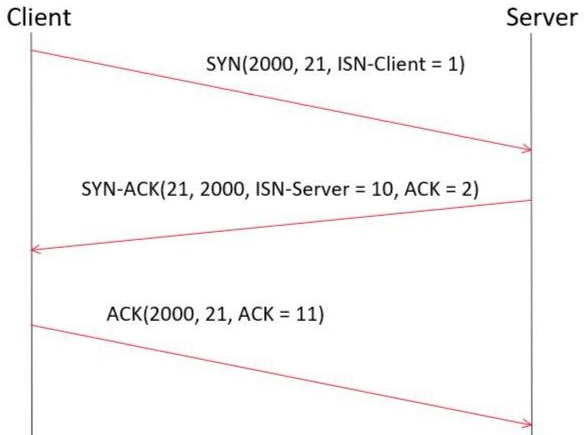
\includegraphics[width=0.5\textwidth]{ConnectionSetup_12062019}
		\end{figure}
		Il primo pacchetto SYN inviato dal Client contiene:
		\begin{itemize}
			\item Porta sorgente: 2000 (generato casualmente)
			\item Porta destinazione: 21 (porta FTP)
			\item Sequence Numerber: 1 (generato casualmente)
		\end{itemize}
		Il pacchetto SYN-ACK inviato dal Server contiene:
		\begin{itemize}
			\item Porta sorgente: 21 (porta FTP che fornisce il servizio richiesto)
			\item Porta destinazione: 2000 (porta del Client che ha richiesto il servizio)
			\item Sequence Numerber: 10 (generato casualmente)
			\item ACK: 2 (Sequence number inviato dal Client incrementato di 1 per specificare a quale pacchetto fa riferimento e ha ricevuto)
		\end{itemize}
		L'ultimo pacchetto inviato dal Client:
		\begin{itemize}
			\item Porta sorgente: 2000 
			\item Porta destinazione: 21 
			\item Sequence Numerber: 2 (generato casualmente)
			\item ACK: 11 (Sequence number inviato dal Server incrementato di 1 per specificare a quale pacchetto fa riferimento e ha ricevuto)
		\end{itemize}
	\end{enumerate}
\end{document} 